\chapter{Feature Selection Methods}


\section{Motivation for Feature Selection}
\label{sec:motivation-feature-selection}
% Feature selection method - page 19
One of the fundamental motivations for feature selection is to deal with a \textit{curse of dimensionality}, which refers to a collection of phenomena that arise when analyzing data in high-dimensional spaces, where the number of features 
$p$ is large. In such settings, the geometry of the space changes in a way that makes many standard statistical and machine learning methods less effective.

As illustrated by the authors in  \cite{hastie2001}; the curse of dimensionality becomes particularly clear when analyzing how neighborhoods behave in high-dimensional spaces. Consider inputs uniformly distributed in a 
$p$-dimensional unit hypercube $[0,1]^p$, as in Figure~\ref{fig:hypercube}. We define a local neighborhood as a smaller $p$-dimensional hypercube, such that it contains a fixed fraction $r \in (0,1)$ of the total volume of the space.

To achieve this, the edge length of the neighborhood hypercube must satisfy
\begin{equation}
    \varepsilon_p(r) = r^{1/p}.
\end{equation}

This relationship has a counterintuitive implication: as the dimension $p$ increases, the required edge length grows rapidly. In particular, the side length $\varepsilon_p(r)$ approaches $1$ as $p \to \infty$, even for small values of $r$. This means that to capture a fixed proportion of the data, one must include a large fraction of each variable’s range.

For example, in ten dimensions, retaining only $1\%$ of the total volume requires an edge length of $0.01^{1/10} \approx 0.63,$
while retaining $10\%$ requires approximately $0.1^{1/10} \approx 0.80.$ 

This phenomenon highlights a key issue in high-dimensional data analysis: points that are in low-dimensional settings may become effectively distant when embedded in higher-dimensional spaces. As a consequence, data becomes increasingly sparse, meaning that most regions of the space contain few or no observations. This sparsity makes local methods less reliable and significantly complicates tasks such as distance-based learning, clustering, and density estimation in high dimensions.

\begin{figure}[ht]
    \centering
    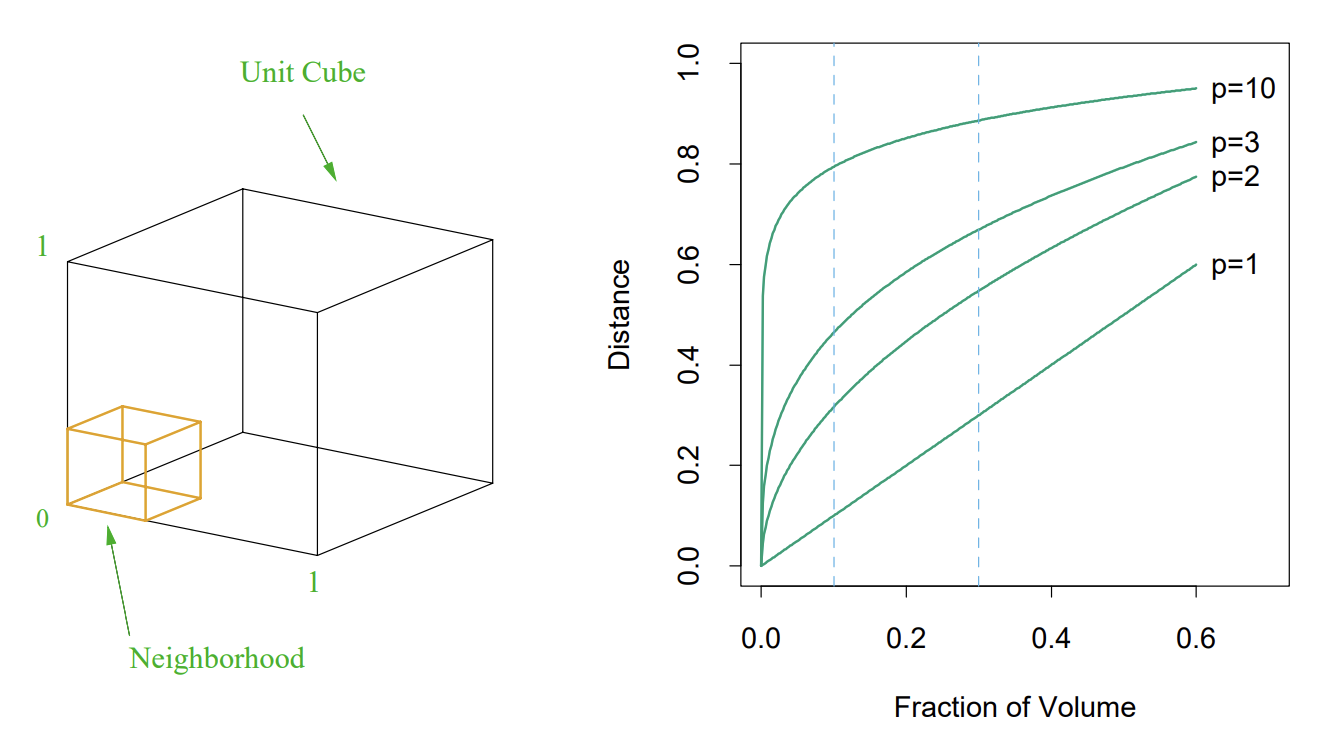
\includegraphics[width=0.8\textwidth]{figures/image.png}
    \caption{Illustration of the curse of dimensionality. Reproduced from \cite{hastie2001}.}
    \label{fig:hypercube}
\end{figure}

\section{Feature Selection: Formal Definition and Feature Types}

\url{https://ift6758.github.io/lectures/feature_selection.pdfx}

\emph{Feature selection} addresses these issues by reducing the dimensionality of the input space.

Let $(\mathbf{X}, Y) \sim P$, where $\mathbf{X} \in \mathbb{R}^p$ is a random vector of features and $Y$ is the target variable. Let $P$ denote their joint probability distribution.

Realizations of $\mathbf{X}$ and $Y$ are denoted by $\mathbf{x} = (x_1, \dots, x_p) \in \mathbb{R}^p$ and $y$, respectively.

The goal of feature selection is to identify a subset of feature indices $S \subseteq \{1, \dots, p\}$ such that $|S| = k \ll p$. For a given subset $S$, define the reduced random feature vector
\[
\mathbf{X}_S = (X_j)_{j \in S},
\]
whose realization is denoted by $\mathbf{x}_S \in \mathbb{R}^k$, obtained by selecting the components of $\mathbf{x}$ indexed by $S$. The learning algorithm is then applied to \( \mathbf{x}_S \) instead of the full feature vector \( \mathbf{x} \).

The goal of feature selection is to identify informative features and remove those that do not contribute to prediction.

A feature \( X_j \) is said to be \emph{relevant} if it provides additional information about \( Y \), i.e.
\begin{equation}
P(Y \mid \mathbf{X}) \neq P(Y \mid \mathbf{X}_{-j}),
\end{equation}
where \( \mathbf{X}_{-j} \) denotes the random vector with the \( j \)-th component removed.

A feature \( X_j \) is \emph{irrelevant} if it does not affect the conditional distribution of \( Y \), i.e.
\begin{equation}
P(Y \mid \mathbf{X}) = P(Y \mid \mathbf{X}_{-j}).
\end{equation}

A feature \( X_j \) is \emph{redundant} if its information is fully contained in a subset of other features \( S \subseteq \{1, \ldots, p\} \setminus \{j\} \), i.e.
\begin{equation}
P(Y \mid X_j, \mathbf{X}_S) = P(Y \mid \mathbf{X}_S).
\end{equation}

Removing irrelevant features reduces noise, while removing redundant features eliminates unnecessary duplication of information. Both contribute to a more compact and efficient representation of the data.

\section{REMOVE}
Feature selection is a key approach to mitigating the curse of dimensionality, as it reduces the number of irrelevant or redundant variables and simplifies the learning problem. By lowering the number of features, the hypothesis space becomes significantly smaller, improving both computational efficiency and model performance \cite{mitchell1997, goodfellow2016}.

For example, with $n$ binary features and a binary label, the size of the hypothesis space is  \[2^{2^n}\]. If each feature can take $m$ values and the class has $l$ labels, the hypothesis space grows even faster to \[l^{m^n}\]. This illustrates how rapidly complexity increases with dimensionality.

Reducing the number of features also improves data coverage. For a fixed number of training instances $m$, decreasing $n$ increases the ratio $m / 2^n$, meaning that the input space is more densely populated. For instance, reducing from $n = 10$ to $n = 5$ leads to a substantial increase in coverage. This significantly improves the representativeness of the training data and allows learning algorithms to generalize more reliably \cite{liu2007}. 






\section{Feature Selection vs.\ Feature Extraction}

Feature selection and feature extraction are two approaches to dimensionality reduction.

\subsection*{Common properties}

Both feature selection and feature extraction aim to reduce the dimensionality of the data, which decreases storage and computational requirements. By simplifying the input space, they can improve the performance of learning algorithms, particularly in high-dimensional settings. Additionally, both approaches support the construction of models that generalize better to unseen data.

Common feature selection methods include filter approaches such as mutual information and correlation-based selection, wrapper methods that evaluate subsets of features using predictive models, and embedded methods like Least Absolute Shrinkage and Selection Operator (LASSO) or decision tree–based selection. These approaches will be discussed in more detail in \textcolor{blue}{Section 2.4}. 

Common feature extraction methods include principal component analysis (PCA), independent component analysis (ICA), linear discriminant analysis (LDA), and autoencoders. While the underlying approaches differ, both families of methods aim to capture the most relevant information in a smaller representation of the data.

\subsection*{Differences}

The key difference lies in how the reduced representation is constructed.

Feature selection chooses a subset of the original features. Formally, it defines a projection
\[
\pi_S : \mathbb{R}^p \to \mathbb{R}^k, \quad \pi_S(x) = (x_j)_{j \in S}.
\]
The original variables are preserved, which maintains their physical meaning and allows direct interpretation of the model.

Feature extraction constructs new features as transformations of the original ones. It defines a mapping
\[
\phi : \mathbb{R}^p \to \mathbb{R}^k,
\]
where the components of $\phi(x)$ are typically functions of all input variables (e.g.\ linear combinations). In this case, the original meaning of individual features is generally lost.

As a result, feature selection is preferred when interpretability is important, while feature extraction is more suitable when the goal is maximal dimensionality reduction or capturing complex structure in the data.

\section{Applications of Feature Selection}
Feature selection becomes particularly important in datasets with high dimensionality, noisy features, or a small number of samples relative to the number of features. High-dimensional datasets often contain irrelevant or redundant features, which can reduce model performance and increase computational cost. 
For example, in genomics, a single experiment can measure tens of thousands of gene expression levels for only a few hundred samples. In such cases, most features are either irrelevant or occur with very low frequency, making it difficult for learning algorithms to identify meaningful patterns. 
Similarly, text classification datasets may contain thousands of words that contribute little to the predictive task. Feature selection mitigates these issues by identifying a subset of informative and non-redundant features.

\section{Feature Selection Algorithms}
\textbf{Based on label availability} \\
Feature selection methods can be classified by whether they use label information during selection. \emph{Supervised methods} rely on labeled data to identify features that best predict the target, as in classification or regression. \emph{Unsupervised methods} do not use labels and instead select features based on intrinsic properties of the data, such as variance or similarity, making them suitable for clustering or exploratory analysis. \emph{Semi-supervised} methods combine labeled and unlabeled data, exploiting the small amount of labeled information while leveraging the structure in the unlabeled data. In this thesis, we focus exclusively on supervised feature selection methods.  

\textbf{Based on output type} \\
Feature selection methods can also be categorized according to the form of their output. Some methods return a \emph{subset of features}, typically represented as a vector of selected feature indices. Others produce a \emph{rank of features}, often as an ordered list indicating their relative importance. A third type of output consists of \emph{feature weights}, where each feature is assigned a relevance score; these weights can subsequently be used to derive a ranking by ordering features according to their values.

\textbf{Univariate or multivariate methods} \\
Feature selection methods can also be classified as univariate or multivariate (Lazar et al., 2012). Univariate methods evaluate each feature independently with respect to the target variable, ignoring dependencies between features. These approaches are typically simple and computationally efficient, but they may fail to capture feature interactions. In contrast, multivariate methods evaluate features jointly and account for dependencies among them. While these methods are generally more complex, they tend to be more robust as they can capture feature interactions and synergy.

\textbf{Selection strategies} \\
From the perspective of selection strategy, feature selection algorithms can be categorized into wrapper, filter, and embedded methods, with additional approaches including hybrid and ensemble methods ([1]).

\subsection{Wrapper methods} 
Wrapper methods perform a search over the space of possible feature subsets to find the one that optimizes a predictive model’s performance. Formally, each candidate subset \(S \subseteq \{1, \dots, p\}\) is assessed using a cost function \(\mathcal{L}(S)\), which typically represents a measure of prediction error. Common choices include misclassification error \textcolor{red}{need to be established}need to be established), mean squared error, or cross-validated risk. For example, in a general setting the cost function can be written as

\[
\mathcal{L}(S) = \frac{1}{n} \sum_{i=1}^{n} \ell\big(y_i, f_S(x_i)\big),
\]
where \(\ell(\cdot, \cdot)\) is a loss function, \(x_i\) denotes the feature vector restricted to the subset \(S\), and \(f_S\) is the model trained using only the features in \(S\).

Here, \(f_S\) is trained on the features in \(S\). The objective of the wrapper method is then to find the subset that minimizes this cost function:
\[
S^* = \min_{S \subseteq \{1, \dots, p\}} \mathcal{L}(S).
\]

These methods evaluate subsets according to a search strategy, which determines the order and selection of candidate subsets. These methods proceed iteratively: in each step, a candidate subset is evaluated, and the search is updated accordingly. Iterations continue until a stopping criterion is satisfied, such as a maximum number of iterations or a minimal improvement in model performance. Search strategies vary, and some of them will be discussed in the next section.

 Wrappers can be applied to any model but are computationally expensive. The main drawback of wrappers is that each subset evaluation requires training and predicting at least one model, which significantly increases computational cost \cite{ang2015}. In this thesis, we examine SVM Recursive Feature Elimination (SVM-RFE) as an example of a wrapper method. 

\subsection{Filter methods}
Filter methods are independent of any learning algorithm and rely on intrinsic properties of the data. They usually rank or score features using statistical or information-theoretic criteria such as correlation, chi-squared statistics, mutual information, or information gain. Filter methods are computationally efficient and often serve as a preprocessing step.

Some of the Filter methods

 The main difference lies in the scoring function.
In filtering approaches, the cost function is defined in terms of data
intrinsic characteristics. In contrast, in wrapper approaches, the cost
function is based on the predictive error of a single classifier

In this thesis, we discuss Kruskal--Wallis, Mutual Information, ReliefF, and mRMR as representative filter methods.

\subsection{Embedded methods}
Embedded methods perform feature selection during the training of the model. These methods are part of the model either as built-in functionality or via regularization. Common embedded approaches include decision tree--based algorithms such as Classifcation and Regression Trees (CART), and Random Forest, as well as variants of multinomial logistic regression. Some embedded methods apply regularization to perform feature weighting, forcing coefficients to shrink or become exactly zero, as in LASSO or Elastic Net. Embedded methods inherit the merits of wrapper and filter methods: they account for feature interactions with the learning algorithm and are generally more efficient than wrappers. 


\section{Search strategies}
A \textit{search strategy} defines the order in which the variable subsets are evaluated. These strategies are particularly important for wrapper methods. Few of the search strategies are proposed by Guyon et al. \cite{guyon2006}. Most common strategies are forward selection, backward elimination, floating search, and randomized search. 

\textit{Forward selection} starts with an empty feature set and adds features one at a time, keeping those that improve the model's performance. \textit{Backward elimination} starts with all features and removes them iteratively, discarding those that contribute least to the predictive power.

Both methods are considered exhaustive searches, as they evaluate all possible subsets of features up to a certain size. For datasets with many features, forward and backward selection can be computationally expensive. In forward selection, if the optimal number of features $k$ is unknown, one may need to evaluate all subsets of size $1$ to $k$, requiring $\binom{N}{1} + \binom{N}{2} + \dots + \binom{N}{k}$ combinations, which gives a time complexity of $O(2^N)$. 

For this reason, more efficient algorithms have been developed, such as sequential forward selection (SFS) and sequential backward selection (SBS). SFS starts with an empty feature set and iteratively adds the feature, that yields the greatest improvement in model performance, while previously selected features remain selected. SBS is similar to SFS, but it starts with the full feature set and iteratively removes the feature that contributes the least. Both SFS and SBS are heuristic, thus they do not guarantee the optimal subset. Research also shows that exhaustive search is more prone to overfitting, than sequential methods. \textcolor{red}{[add citation or reference]}

\emph{Floating search} extends forward or backward selection by allowing conditional inclusion or exclusion of features. \emph{Sequential Forward Floating Selection} (SFFS) can remove previously added features if they later become redundant, and \emph{Sequential Backward Floating Selection} (SBFS) can re-add previously removed features, making the search more flexible.

\emph{Randomized search} explores the subset space probabilistically, using heuristics or metaheuristics such as genetic algorithms.


\section{HILBERT SCHmidt}
\section*{Hilbert-Schmidt Independence Criterion Lasso Based Feature Selection}

For high-dimensional and small sample data (e.g., dimensionality $> 10^5$ and the number of samples $< 10^3$), the Hilbert-Schmidt Independence Criterion Lasso (HSIC Lasso) is useful.

The HSIC Lasso optimization problem is given by:
\[
\mathrm{HSIC\text{-}Lasso}:\quad
\min_{\mathbf{x}} \;
\frac{1}{2} \sum_{k,l=1}^{n} x_k x_l \,\mathrm{HSIC}(f_k, f_l)
- \sum_{k=1}^{n} x_k \,\mathrm{HSIC}(f_k, c)
+ \lambda \|\mathbf{x}\|_1
\]
subject to
\[
x_1, \ldots, x_n \geq 0.
\]

Here,
\[
\mathrm{HSIC}(f_k, c) = \mathrm{tr}(\bar{\mathbf{K}}^{(k)} \bar{\mathbf{L}})
\]
is a kernel-based independence measure called the empirical Hilbert-Schmidt Independence Criterion (HSIC), where $\mathrm{tr}(\cdot)$ denotes the trace and $\lambda$ is the regularization parameter.

The centered Gram matrices are defined as:
\[
\bar{\mathbf{K}}^{(k)} = \mathbf{\Gamma} \mathbf{K}^{(k)} \mathbf{\Gamma}, 
\qquad
\bar{\mathbf{L}} = \mathbf{\Gamma} \mathbf{L} \mathbf{\Gamma},
\]
where
\[
K^{(k)}_{i,j} = K(u_{k,i}, u_{k,j}), 
\qquad
L_{i,j} = L(c_i, c_j),
\]
and $K(\cdot,\cdot)$ and $L(\cdot,\cdot)$ are kernel functions.

The centering matrix is given by:
\[
\mathbf{\Gamma} = \mathbf{I}_m - \frac{1}{m} \mathbf{1}_m \mathbf{1}_m^T,
\]
where $\mathbf{I}_m$ is the $m$-dimensional identity matrix, and $\mathbf{1}_m$ is the $m$-dimensional vector of ones.

The $\ell_1$-norm is denoted by $\|\cdot\|_1$.

HSIC always takes a non-negative value and is zero if and only if two random variables are statistically independent when a universal reproducing kernel such as the Gaussian kernel is used.

The HSIC Lasso can equivalently be written as:
\[
\mathrm{HSIC\text{-}Lasso}:\quad
\min_{\mathbf{x}} \;
\frac{1}{2} \left\| \bar{\mathbf{L}} - \sum_{k=1}^{n} x_k \bar{\mathbf{K}}^{(k)} \right\|_F^2
+ \lambda \|\mathbf{x}\|_1
\]
subject to
\[
x_1, \ldots, x_n \geq 0.
\]

Here, $\|\cdot\|_F$ denotes the Frobenius norm. The optimization problem is a Lasso problem and can be efficiently solved using modern optimization methods such as the dual augmented Lagrangian method.


\section{Properties of Feature Selectors}

